\textbf{Estimating $\bm{C_{gag'a'y}}$:}
\# daily type-$y$ contacts per-person from patch/age $ga$ to patch/age $g'a'$:
\bigskip\par
\begin{minipage}{.65\linewidth}
  \begin{itemize}
    \item Define two types of ``mixing pools'' (Figure~\ref{fig:pools}):
    \begin{enumerate}[leftmargin=2.5ex]
      \item \textbf{Home pools:} can only contact other residents of this patch
      \item \textbf{Travel pools:} can contact anybody currently present
    \end{enumerate}
    \item For each contact type $y$ \& patch $\g$:
    \begin{itemize}
      \item Population from $g'$ present in travel pool: $P^{\,\g}_{g'a} = B_{g'\g} P_{g'a}$
      \item Adjust age contact patterns $C_{aa'y}$ to $P^{\,\g}_{g'a}$ per \cite{Arregui2018}
      \item Assume random mixing by patch $gg'$ within pool
    \end{itemize}
    \item Assume reduced mobility $\rightarrow$ reduced non-home contacts
    \item Sum contacts from all patch $\g$ pools $\rightarrow$ Total contacts $C_{gag'a'y}$
%    \item Force of infection among $ga$: aggregate across $g'$, $a'$, and $y$
  \end{itemize}
\end{minipage}\hfill%
\begin{fig}{.35\linewidth}\null
  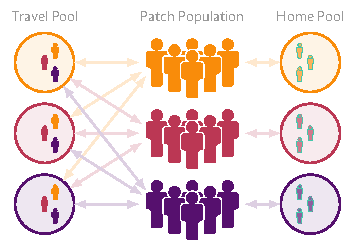
\includegraphics[width=\linewidth]{pools}
  \caption{Illustration of travel vs home mixing pools for 3 toy patches}
  \label{fig:pools}
\end{fig}
\medskip\par
\paragraph{Experiment:}
We estimated \& compared (subtracted) $C_{gag'a'y}$ under different sets of assumptions:
\bigskip\par
\begin{tabular}{crcll}
  \textbullet & (\ass1+\ass2+\ass3) & subtract & (\ass2+\ass3) & $\enspace\rightarrow\enspace$ assumption \ass1 effect \\
  \textbullet &       (\ass2+\ass3) & subtract & (\ass3)       & $\enspace\rightarrow\enspace$ assumption \ass2 effect \\
  \textbullet &             (\ass3) & subtract & ($\cdot$)     & $\enspace\rightarrow\enspace$ assumption \ass3 effect
\end{tabular}
\bigskip\par
We aggregated $C_{gag'a'y}$ across patches/ages to show overall patterns by age $aa'$ or patch $gg'$